\chapter*{Opleiding}

\begin{figure}[h]
    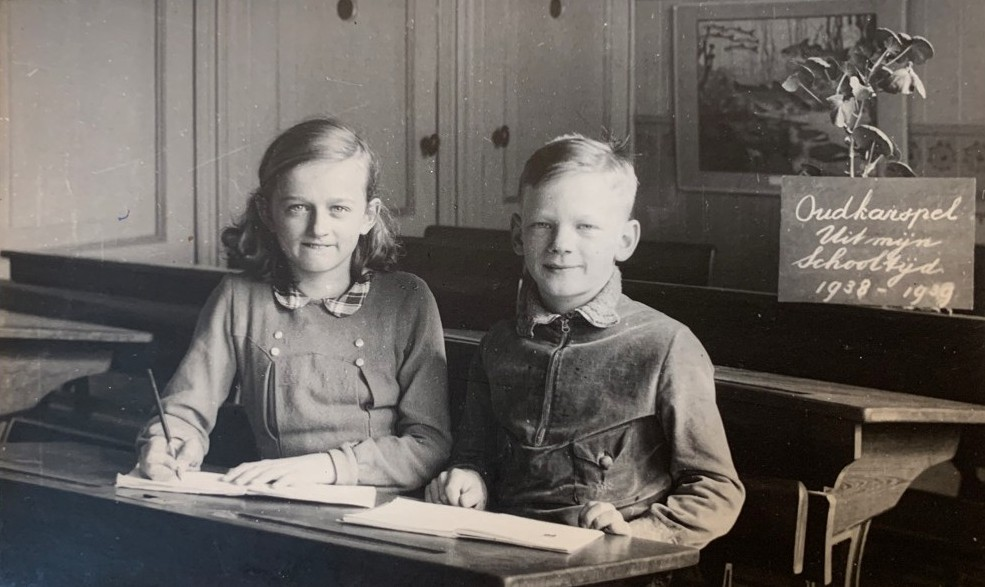
\includegraphics[width=\textwidth]{image26}
    \caption{Tine en Kees, schoolfoto 1938-1939.}
\end{figure}

Het grootste gedeelte van mijn basisschooltijd woonde ik in Oudkarspel. Toen was het zo dat je niet naar de kleuterschool ging, school begon toen je 6 jaar oud was. 

Ik ben naar een openbare lagere school gegaan, het was de enige school in het dorp, mijn vader had ook op deze school gezeten. Naar mijn idee was het een hele grote school met veel ruimte om te spelen. Er was ook een waterput, mijn vader vertelde dat hij als kind daar altijd overheen sprong, dat was een spelletje. Ik kon me dat niet zo goed voorstellen hoe dat dan moest. 

Van de lagere school kan ik me herinneren dat de eerste en de tweede klas in hetzelfde lokaal zaten en ik altijd naar het bord van de tweede klas zat te kijken. Lezen kon ik eigenlijk al voordat ik naar school ging en daarom vond ik het in eerste klas een beetje saai. Rekenen vond ik niet zo leuk, ik was meer van de talige vakken en aardrijkskunde en geschiedenis. 

Op school zat ik veel te lachen. Ik zat meestal naast een vriendin met wie ik altijd aan het giebelen was, hierdoor werden we een keer uit elkaar gehaald en moesten we beide in aan de andere kant van het lokaal zitten. Ik vond het leuk om naar school te gaan. 

We gingen lopend en ik nam vaak mijn (ijzeren) hoepel mee, hier sloeg je tegenaan met een stok zodat ie ging rollen. Als de bel ging dat stond je allemaal voor de klas in de rij te wachten totdat de juf of meester je naar binnen liet. In die tijd gingen veel kinderen met klompen naar school, hier stond dan een bak voor klaar in het schoolgebouw. Ik had meestal geen klompen aan omdat ik ze niet prettig vond zitten. 

In 1939 zijn we naar Schoorl verhuisd, hier heb de 6\textsuperscript{e} klas van de lagere school gevolgd. In Schoorl zat ik op een geheel nieuwe school. Ik kan me nog herinneren dat ze daar rekenboekjes hadden met de antwoorden achterop, zodat je kon controleren of je het antwoord goed had: (lachend) Ik controleerde heel veel.

Ik vond het verhuizen naar Schoorl niet zo erg, ik vond het daar veel leuker dan in Oudkarspel vanwege de duinen en het strand. Tijdens de bezetting mochten we alleen niet naar het strand, voor het geval de Engelsen kwamen. 

\begin{figure}[h]
    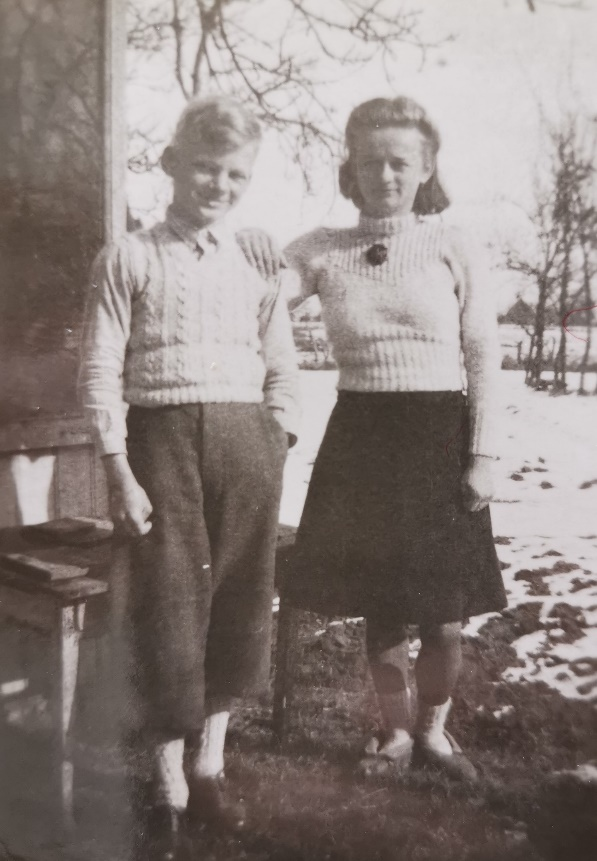
\includegraphics[width=0.9\textwidth]{image27}
    \caption{Tine en Kees.}
\end{figure}

Na de basisschool ben ik naar de Mulo in Bergen gegaan, dit was een opleiding van 4 jaar. Het was toen oorlog dus ik heb deze school nooit van binnen gezien. In het schoolgebouw zaten de Duitsers dus daar konden we niet meer zijn. We zaten toen tijdelijk in een ander schoolgebouw. 

Ik kan me herinneren dat er dat er eens Duitsers op dat schoolplein aan het oefenen waren, de meester heeft ze toen uitgelegd dat het voor te veel afleiding zorgde voor de leerlingen en waarachtig hoor, ze gingen weg. Ik weet nog dat we dat geweldig vonden.

Op een gegeven moment ben ik gestopt met die school want toen lagen we vaker in de berm vanwege de beschietingen door de geallieerden dan dat we in de klas zaten. Pas na de bevrijding heb ik het afgemaakt.

Na de Mulo ben ik naar huishoudschool in Alkmaar gegaan om de huishoudkundige opleiding te volgen. Hier werd je opgeleid tot leidinggevende van bijvoorbeeld het schoonmaakpersoneel in een instelling. Dit was een tweejarige opleiding. 

Ik moest dan ‘s morgens met de bus (die heel vol was, ook met Duitsers) die gestookt werd met hout. Er hing dan een karretje achter de bus waar dit gestookt werd zodat de bus kon blijven rijden, vanwege de oorlog was er geen benzine meer. Ik moest dan vroeg opstaan en ik was niet zo van het ‘’leuk vroeg opstaan’’ maar je deed het gewoon, dit was nou eenmaal zo. 

Bert had wel verder kunnen gaan studeren. Dat wou m’n vader graag. Bert wou dat niet; hij wou trouwen! Na de oorlog zijn ze getrouwd vlak voordat ik naar Engeland ging.

Werken in het Wilhelmina Gasthuis

Ik ben tot mijn 19\textsuperscript{e} naar school gegaan. Hierna heb ik even in Bergen gewerkt in een huis waar groepen jongeren kwamen voor lezingen en studie (voor als je dominee wil worden) in de grote keuken gewerkt. Ik kookte dan samen met een paar kinderen voor deze groepen en ik regelde de bestellingen. 